% !TeX root = ../Bachelorarbeit.tex
\chapter{Auswertung}
Das Passwort war jahrzehntelanger Vorherrscher in der Authentifikation im Web und schien eine kurze Weile auch sicher. Nach dem die ersten Bruteforce-Angriffe auf Formulare angeggangen wurden, mussten neue Regeln für Passwörter her. Der Nutzer durfte sie nicht mehr nach eigenem Ermessen wählen, da der Imageschaden durch z.B: die Infiltrierung einer wichtigen hochrangigen Person eines Unternehmens zu groß wurde. Die Fälle der Data-Breaches und Leaks wurden trotz Passwort-Policy Ansätzen und der Einführung des zweiten Faktors nicht weniger sondern im Gegenteil: Sie häuften sich mehr und mehr. Passwörter wurden theoretisch durch erzwungene Sonderzeichen und einer Mindestlänge komplexer, allerdings wurde genau hier nicht mit der Natur des Menschen gerechnet. Da Formulare nun mehr und mehr Passwörter abzulehnen schienen, beggangen Menschen die Sicherheitsfeatures instinktiv zu umgehen. Darauf folgten die 'zeitlich begrenzten Passwörter', welche aus dem selben Grund, dem Bequemlichkeitsproblem, scheiterten. Neuere Verfahren sollten die alteingesessenen ersetzen oder zunächst ein Mal unterstützen. Die neue Zeit des Smartphones ermöglichte den Nutzern ihre Geräte zur Authentifikation zu nutzen, wofür sie davor kostspielige Geräte kaufen hätten müssen. Die Zeit der Einmalkennwörter brach an und Apps wie der Google Authenticator oder der Microsoft Authenticator gewannen mehr und mehr an Popularität. Mit der Zeit wurden allerdings auch diese 'weiteren Schritte' zur Authentifikation dem Nutzer zu lästig. Vor allem wichtige Dienste wie Banken führen kein Sessionmanagement und nötigen den User häufig zur mehrmaligen Authentifikation während einer Sitzung. Und genau an diesem Standpunkt setzen die neuesten Verfahren an. Die Webauthentikation ist dem Passwort in vielen Dingen überlegen. Zunächst ein Mal werden nur noch zufällig generierte Schlüssel ausgetauscht. Außerdem geschieht das über Challenge-Response-Verfahren wodurch Wiederholungsangriffe vermieden werden. Der Nutzer ist nicht mehr der Kern der Authentifikation sondern der Authentifikator (das Gerät) selbst. Bei neueren public-private-key Verfahren gibt es keine Geheimnisse, die auf einfachste Art und Weise (z.B: über Keylogger, Trojaner oder Shoulder Surfing) entwendet werden könnten. Die Verantworung zur sicheren Aufbewahrung von Passwörtern hat sich vom Nutzer auf die Betriebssysteme verschoben, die die privaten Schlüssel sichern müssen. Die \ac{mitm} - Problematik schien immernoch nicht gelöst. So ist die Kommunikation dann durch den \ac{mitm} angreifbar, wenn der Aussteller des Zertifikats nicht bekannt ist. Die Webauthentikation bietet einem Mann in der Mitte allerdings keine einfache Möglichkeit, die Identität des Nutzers anzunehmen.
\newpage

Abseits der Problematik bietet der FIDO2 - Standard mit Webauthn und CTAP2 die Kommunikation über verschiedenste Authentifikatoren und bietet damit potenziell sehr vielfältige Lösungsansätze für Authentifikationen im Webbereich.
Dennoch ist die Umsetzung des Hauptbetriebssystems Windows aus UX-Sicht nur suboptimal. Gleichzeitig ist die Implementation von Webauthn auf Clientseite zwar größtenteils schon möglich, auf Serverseite fehlt es bei Javascript basierenden Webseiten aber an ausgereiften Web-API's. Die Abstraktion der Vorgänge im Webauthn - Protokoll durch vorhandene API's (wie die genutze im Prototyp) hat den Vorteil, dass der Implementationsaufwand durch eine Senkung der Komplexität sinkt. Gleichzeitig muss bei Fehlern in der abstrahierten Bibliothek ein Mehraufwand an Verständnis dessen, was die Bibliothek macht, aufgetrieben werden. Gemessen daran, dass man das Protokoll allerdings nur einmalig implementieren muss und die FIDO-Alliance große Unterstützung für Webseiten für alle möglichen Programmiersprachen bietet, scheint dieses Argument entkräftigt. Wichtig ist es nun, neben Sicherheit und Bequemlichkeit einen Blick auf den Datenschutz zu werfen, dazu wurde die Checkliste vom IT-Grundschutz für Webseiten ausgefüllt und wird im Folgenden erläutert.

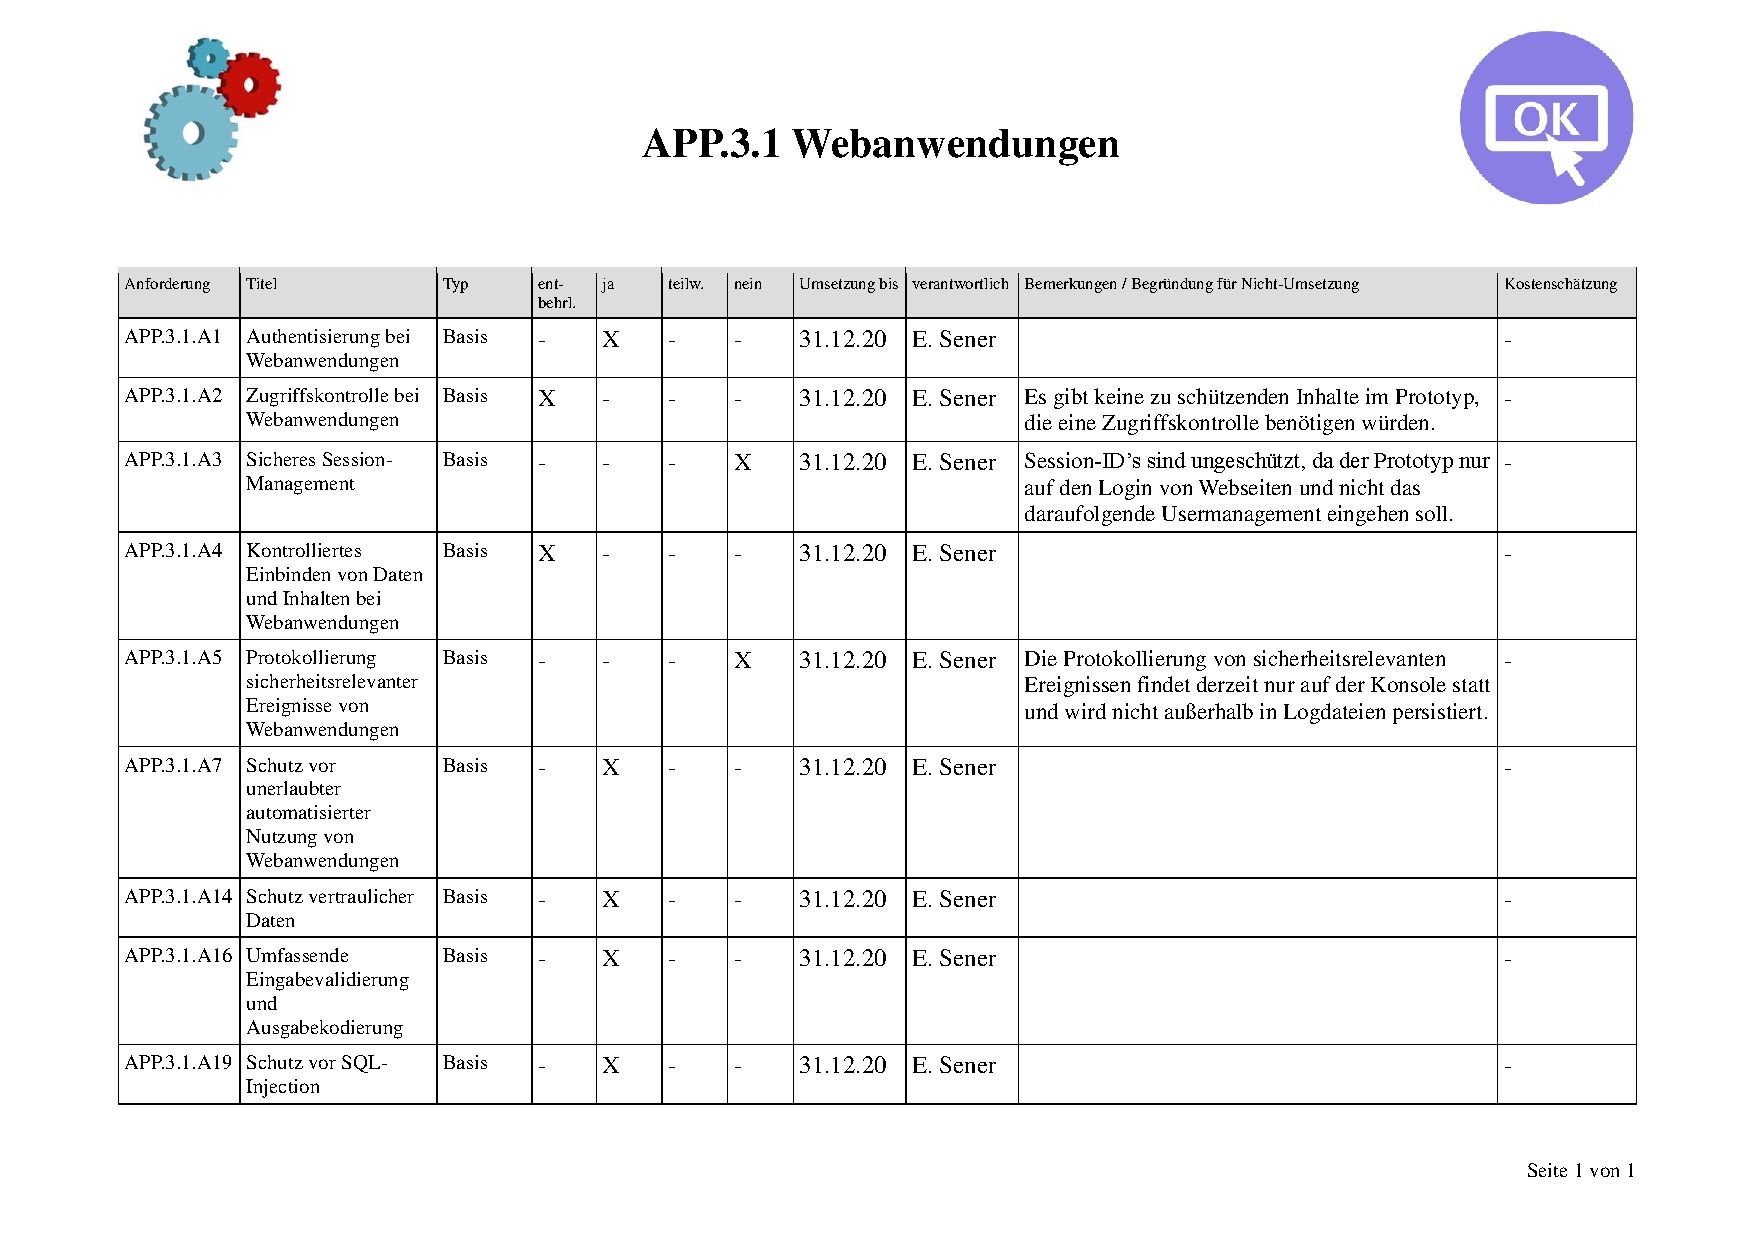
\includepdf[scale=1.0, pages=1]{Documents/ITGS_Webanwendungen.pdf}

Ein grober Blick auf die Anforderungen das IT-Grundschutzes für eine Basisabsicherung ergaben zudem, dass die meisten Punkte umgesetzt werden konnten. Woran es der Anwendung weiterhin fehlt ist eine weiterführende Protokollierung von sicherheitsrelevanten Ereignissen sowie dem bereits erwähnten Session-Management. Grundsätzliche Bedrohungen wie \ac{mitm} - Angriffe und SQL - Injektionen wurden bei der Implementation bedacht und werden bereits verhindert. Eine Zugriffskontrolle schien für den Prototypen entbehrlich, da keine zu schützenden Daten verwendet werden und deshalb zum jetzigen Stand der Anwendung keine Kontrolle über den Zugriff auf diese nötig ist.

Der Prototyp beweist zweierlei Dinge. Zunächst ein Mal ist es möglich, einen Nutzer bereits mit einem einzigen sicheren Faktor und dessen Nutzernamen zu authentifizieren. Das Passwort sollte im Jahre 2020 eher zur Ausnahme in der Sicherung und wenn überhaupt nur mit einem zweiten Faktor verwendet werden dürfen, sofern es dem User nicht möglich ist die sichereren Verfahren zur Authentifikation zu nutzen. Dies könnte zum Beispiel dann der Fall sein, wenn es dem Nutzer an den benötigten Geräten (der Hardware) fehlt oder die Hardware nicht mit dem Betriebssystem kompatibel ist. Außerdem beweist die Webseite, dass die Implementation der neueren Verfahren keine große Hürde darstellt und einem potenziellen Unternehmen auf lange Sicht viele Supportanfragen zwecks vergessenen Passwörtern oder gekaperten Accounts ersparen kann.

Zum Ende der Facharbeit muss noch geklärt werden, welches Verfahren für welchen Nutzertypus geeignet ist. Auch wenn man dies nicht pauschalisieren kann, sollte man zunächst ein Mal klären welcher Nutzer welche Anforderungen stellt. Alle Internetnutzer, ob es nun ein erfahrener Entwickler, ein Casual Erwachsener oder Jugendlicher ist, haben Interesse an dem Schutz ihrer Daten. Auch wenn ihnen die Wichtigkeit ihrer Daten und die Gefährdung größenteils nicht bewusst sind. Jugendliche haben heutzutage nur in seltenen Fällen kein Smartphone und können somit das TOTP-Verfahren oder die Webauthn (falls von der Internetseite umgesetzt und untersützt) verwenden. Älteren Personen fehlt es womöglich an technischer Hardware, doch hier kommt die Authentifikation über PIN (sogenanntes self-signed-device) oder die Stimme am Rechner ins Spiel. Auch wenn kein externes Gerät wie ein Smartphone vorhanden ist, kann häufig bereits der eigene Rechner einige Authentifikationsmethoden unterstützen. Sollte man, aus gegebenen und teilweise genannten Gründen, keine Möglichkeit auf Alternativen zum Passwort besitzen, sollte das Passwort nicht als alleiniger Authentifikator verwendet werden dürfen. Ein zweiter Faktor ist aber nur strikt für das Passwort erforderlich, denn die anderen Verfahren sind nicht so großen Gefahren ausgesetzt wie es das Passwort ist. Die Öffentlichkeit muss sich der Wichtigkeit ihrer Identität bewusst werden, um die Entscheidung über Passwörter und dem erzwungenen zweiten Faktor nachzuvollziehen. Zuletzt bleibt noch zu erwähnen: Der Codename des Prototypen 'clsec' ist ein Kürzel der Wortschöpfung 'Clientless Login' und bedeutet so viel wie ``Die Authentifikation ohne Passwort'' und ist gleichzeitig ein Beweis dafür, dass diese auch Zukunft hat.
